\documentclass{article}
\newcommand{\beq}{\begin{equation}}
\newcommand{\eeq}{\end{equation}}
\newcommand{\ber}{\begin{eqnarray}}
\newcommand{\eer}{\end{eqnarray}}
\newcommand{\nn}{\nonumber}
\newcommand{\dd}[2]{\frac{d}{d{#2}}{(#1)} }
\newcommand{\ddeps}{\frac{d}{d\epsilon}\Big{|}_{\rightarrow{0}}}
\newcommand{\pdd}[2]{\frac{\partial{#1}}{\partial{#2}}}
\newcommand{\bD}{{\mathbf{D}}}
\newcommand{\notimplies}{\;\not\!\!\!\implies}
\usepackage{amsmath}
\DeclareMathOperator{\sign}{sign}
\usepackage{amsfonts}
\usepackage{bm}
\usepackage{booktabs}
\usepackage[hyphens]{url}
\usepackage{amssymb} 
\usepackage[utf8]{inputenc} 
%\usepackage[ngerman]{babel} 
\usepackage[T1]{fontenc}
\usepackage[margin=2.5cm]{geometry}
\usepackage{listings}
\usepackage{multirow}
\usepackage{tikz}
\usepackage{cancel}
\definecolor {processblue}{cmyk}{0.96,0,0,0}
\usetikzlibrary {positioning}
\usepackage{hyperref}
% for booktabs
\newcommand{\ra}[1]{\renewcommand{\arraystretch}{#1}}
\begin{document}
\title{Notes from Goodfellow}
\author{Nachiket Gokhale}
\date{\today}
\maketitle
\section{PCA Section 2.12}
Given a decoder $\pmb{D}$, what should the encoder be? The idea is that of all the points $\pmb{c}$ that one could map $\pmb{x}$ to, we should choose the point $\pmb{c}^*$ that minimizes $\|\pmb{x}-g(\pmb{c})\|_2$. Taking derivatives we find that the minimizer satisfies $\pmb{c}^* = \pmb{D}^T\pmb{x}$. So, $\pmb{D}^T$ is our encoder.
\section{Covariance and independence Section 3.8}
\ber
\text{ indepdent variables } & & \implies \text{ zero covariance }\\
\text{ non-zero covariance } & & \implies \text{ dependent variables }\\
\text{ zero covariance }     & & \implies \text{ no linear dependence, can be non-linear dependence }\\
\text{ dependent variables } & & \implies \text{ possible zero covariance, see below}\\
\eer
$\mathrm{x} \in [-1,1]$ be a uniform random variable. Hence, $P(x)=\frac{1}{2}$. $s$ is a discrete random variable taking values $1$ or $-1$ with probability $\frac{1}{2}$. We generate a new random variable $y=sx$. Clearly, $x$ and $y$ are not independent, because $x$ completely determines the magnitude of $y$. However, $\text{Cov}(x,y)=0$. We will prove this. \\
Clearly $x$ and $s$ are independent. Hence,
\beq
\mathbb{E}(y) = \mathbb{E}(xs) = \mathbb{E}(x)\mathbb{E}(s)
\eeq
\beq
\mathbb{E}(x) = \int_{-1}^{1}P(x)xdx = \int_{-1}^{1}\frac{1}{2}xdx = \frac{1}{2}\Big[\frac{x^2}{2}\Big]_{-1}^{1} = 0
\eeq
\beq
\mathbb{E}(s) = P(s=1)1 + P(s=-1)(-1) = 0.5*1+(0.5)*(-1) = 0
\eeq
Therefore $\mathbb{E}(y)=0$
\beq
\text{Cov}(x,y) = \mathbb{E}\Big[(x-\mathbb{E}(x))(y-\mathbb{E}(y))\Big] = \mathbb{E}\Big[xy\Big] = \mathbb{E}\Big[sx^2\Big]
\eeq
Again, since $x$ and $s$ are independent
\beq
\text{Cov}(x,y) = \mathbb{E}\Big[sx^2\Big] =  \mathbb{E}(x^2)\mathbb{E}(s)=0
\eeq
$x$ and $y$ are dependent but their covariance is zero.
Let $x,y$ be independent random variables. Then
\ber
\mathbb{E}(xy) &=& \int \int P(x,y)xy dxy = \int\int P_1(x)P_2(y) xy dxdy \\
               &=& \int P_1(x)xdx \int P_2(y)ydy = \mathbb{E}(x)\mathbb{E}(y)
\eer
I think the critical part is that $P(x,y)=P_1(x)P_2(y)$ if $x,y$ are independent.
\section{ Multinomial/Multinoulli distribution: 3.9.2 }
\subsection{Bernoulli distribution}
Random variable takes value $k=1$ with prob $\theta$ and $k=0$ with prob $1-\theta$. PMF is $\theta^k(1-\theta)^{1-k}$ assuming $0^0=1$. The true mean is
\beq
\theta = 1*P(1) + 0*P(0) = \theta
\eeq
The PMF can be written as
\beq
P(k) = (\theta)^k(1-\theta)^{1-k}
\eeq
From which it can be seen that
\beq
P(0) = (1-\theta) \qquad P(1) = \theta
\eeq
\section{Expectation of a function}
The definition is (equation 3.10) in Goodfellow
\beq
\mathbb{E}(f(x)) = \int f(x) p_x(x) dx
\eeq
If we now want to change the random variable from $x$ to $y=f(x)$ we will need to find a pdf $p_y(y)$, so that we can use the formula
\beq
\mathbb{E}(y)) = \int yp_y(y)dy 
\eeq
$p_y(y) \ne p_x(f^{-1}(y))$. We change variables in the above equation from $y$ to $x$ and get
\ber
\mathbb{E}(f(x)) &= \int f(x)p_x(x)dx \\
               &= \int y p_x(f^{-1}(y)) \frac{dx}{dy} dy
\eer
In the above equation we can identify
\beq
p_y(y) = p_x(f^{-1}(y)) \frac{dx}{dy} 
\eeq
Pretty much a standard change of variables formula.
%
%
%
\subsection{Multinoulli distribution}
From \url{https://www.euanrussano.com/post/probability/multinoulli_multinomial/}.
This distribution is also called categorial distribution, since it can be used to model events with K possible outcomes. Bernoulli distribution can be seen as a specific case of Multinoulli, where the number of possible outcomes K is 2. In machine learning, the multinoullli can used to model the expected class of one sample into a set of K classes. For instance, one may want to predict to which specie  in the set  a flower belongs based on its attribute. Then species K follow a multinoulli distribution.\\
Consider the $p(x=k)$ the probability that the sample $x$ belongs to class k. Here  $x$ could be the attributes of a flower in the example above, or one side of a die in the roll of it. If the set of classes is $K \,\in \, 1,2,3,\cdots,K$ then the probability of each outcome can be written as:
\ber
p(x=1) &=& p_1\\
p(x=2) &=& p_2\\
... & &\\
p(x=K) &=& p_K
\eer
Naturally, the probabilities sum to 1.0. ($\sum_{i}^{K}p(x=i)=1.0$). Coming back to the example of flowers classification, say that for a sample  the following probabilites where obtained for each of the 3 classes.
\ber
p(x=1) &=& 0.1\\
p(x=2) &=& 0.3\\
... & &\\
p(x=K) &=& 0.6
\eer
Clearly $\sum_{i}^{K}p(x=i)=1.0$ and one would say that the sample is most probable from class 3.\\
If we consider 3 classes corresponding to $k=1,k=2,k=3$ then the PMF can be written as
\ber
P(k)=p_1^{(k-2)(k-3)}p_2^{(k-1)(k-3)}p_3^{(k-1)(k-2)}
\eer
Can extend to $n$ classes similarly.
\subsection{Multinomial distribution}
The multinomial distribution describes repeated and independent Multinoulli trials. It is a generalization of he binomial distribution, where there may be K possible outcomes (instead of binary. As an example in machine learning and NLP (natural language processing), multinomial distribution models the counts of words in a document. Similar to Multinoulli, we say that a sample $x$ may take $K$ possible outcomes, each one with prabability $p_K$ after n successive trials. The probability (pmf) of a certain (particular) outcome can be modeled using the formula:
\beq
p(x=k) = \frac{n!}{x_1!x_2!\cdots x_k!}p_1^{x_1}p_2^{x_2}\cdots{p_k^{x_k}}
\eeq
Where $n$ is the number of trials, $x_i$ is the number of times event $i$ occurs and is the probability $p_i$ of event $i$ at each independent trial.\\
As an example, consider a problem which can take 3 outcomes at each trial. The probability of obtaining one specific outcomes can be written as:
\beq
p(x=k) = \frac{n!}{x_1!x_2!x_3!}p_1^{x_1}p_2^{x_2}p_3^{x_3}
\eeq
This can be used to model, for instance, the probability of one specific outcome on a chess tournment. Say that we want to determine what is the probability that, after 12 games, player 1 will have 7 wins, player 2 will have 2 wins and the remaining games will finish in draw. For that, suppose that the probability that Player 1 wins is 0.4, Player 2 is 0.35 and the tie has probability 0.25. Therefore we have,
\ber
n &=& 12\\
x_1 &=& 7\\
x_2 &=& 2\\
x_3 &=& 3 \\
p1  &=& 0.4\\
p2  &=& 0.35\\
p3  &=& 0.25
\eer
Replacing that in the formula shown above:
\ber
p(x=k) = \frac{12!}{7!2!3!}{0.4}^7{0.35}^2{0.25}^3 = 0.0248
\eer
\section{Equation 3.52}
$a$ and $c$ are independent given $b$
\beq
p(a,b,c) = p(a)p(b|a)p(c|b)
\eeq
$p(a,b,c)$ seems to be the probability of $a$ and $b$ and $c$ occurring. The rhs can be simplified to
\beq
p(a,b)p(c|b) = p(a,b)p(c|a,b)  \text{ because of independence}
\eeq
which is the same thing as $p(a,b,c)$.
\section{Equation 5.1}
\beq
p(\mathbf{x}) = p(x_1)p(x_2|x_1)p(x_3|x_1,x_2)
\eeq
RHS =
\beq
p(x_1\cap x_2)p(x_3|x_1x_2) = p(x_1\cap x_2 \cap x_3) = p(\mathbf{x})
\eeq
\section{Biased and unbiased estimators}
Goodfellow equation (5.21) section 5.4.2
The estimator for the mean is
\beq
\hat{\theta}_m = \frac{1}{m}\sum_{i=1}^{m}x^{(i)}
\eeq
Now,
\beq
\mathbb{E}(\hat{\theta}_m) = \frac{1}{m}\sum_{i=1}^{m}\mathbb{E}(x^{(i)})
\eeq
Now
\beq
\mathbb{E}(x^{(i)}) = 1*P(1) + 0*P(0) = \theta \text{ ... } x^{(i)} \text{ can take values 0 or 1 only. }
\eeq
So,
\beq
\mathbb{E}(\hat{\theta}_m) = \frac{1}{m}\sum_{i=1}^{m}\theta = \theta \text{ ...the true mean. Therefore this estimator is unbiased.}  
\eeq
\subsection{Biased estimator for the variance of Gaussian}
From \url{https://dawenl.github.io/files/mle_biased.pdf} Dawen Liang CMU.
The estimator
\beq
\hat{\mu}_{m} = \frac{1}{m}\sum_{i=1}^{m} x^{(i)}
\eeq
is unbiased for the mean of the Gaussian. The biased estimator for the variance of the Gaussian is
\ber
\hat{\sigma}^2_m &=& \frac{1}{m}\sum_{i=1}^{m}(x^{(i)}-\hat{\mu}_m)^2 = \frac{1}{m}\Big[\sum_{i=1}^{m}(x^{(i)})^2 - 2\hat{\mu}_{m}\sum_{i=1}^{m}x^{(i)} + \hat{\mu}_m(m)\Big]\\
&=& \frac{1}{m}\Big[\sum_{i=1}^{m}(x^{(i)})^2 - m\hat{\mu}_m^2\Big] \label{eqn:biasedgaussestim}
\eer
The expected value of this estimator is
\ber
\mathbb{E}(\hat{\sigma}^2_m) = \frac{1}{m}\Big[\sum_{i=1}^{m}\mathbb{E}((x^{(i)})^2)\Big]-\mathbb{E}(\hat{\mu}_m^2)
\eer
Using $\mathbb{E}((x^{(i)})^2)=\mathbb{E}(x^2) \,\,\forall\,\,i$
\beq
\label{eqn:expvargaussestim}
\mathbb{E}(\hat{\sigma}^2_m) = \mathbb{E}(x^2) - \mathbb{E}(\hat{\mu}^2_m)
\eeq
The true variances of $x$ and $\hat{\mu}^2$ are:
\ber
\sigma^2 = \mathbb{E}(x^2) - (\mathbb{E}(x))^2 \implies (\mathbb{E}(x^2) = \sigma^2 + \mu^2 \cdots \text{because } E(x)=\mu\\
\sigma^2_{\hat{\mu}} = \mathbb{E}(\hat{\mu}^2) - \mathbb{E}(\hat{\mu}_m)^2 \implies \mathbb{E}(\hat{\mu}^2_m) =  \sigma^2_{\hat{\mu}} + \mu^2 \cdots \text{because } E(\hat{\mu}_m)=\mu
\eer
Using the above equations in (\ref{eqn:expvargaussestim}),
\beq
\label{eqn:expvargaussestim2}
\mathbb{E}(\hat{\sigma}^2_m)  = \sigma^2 - \sigma^2_{\hat{\mu}}
\eeq
But,
\ber
\sigma^2_{\hat{\mu}_m} &=& \text{var}\Big( \frac{1}{m}\sum_{i=1}^{m} x^{(i)}\Big) \\
&=& \frac{1}{m^2}\text{var}\Big(\sum_{i=1}^{m} x^{(i)}\Big) \\
&=& \frac{1}{m^2}\sum_{i=1}^{m}\text{var}(x^{(i)}) = \frac{1}{m^2}(m\text{var}(x^{(i)}))\\
&=&\frac{1}{m}\text{var}(x^{(i)})= \frac{\sigma}{m}
\eer
Using the above equation in (\ref{eqn:expvargaussestim}),
\beq
\mathbb{E}(\hat{\sigma}^2_m) = \sigma^2 - \frac{\sigma^2}{m} = \Big(1-\frac{1}{m}\Big)\sigma^2
\eeq
Since $\mathbb{E}(\hat{\sigma}^2_m)\ne \sigma^2$, equation (\ref{eqn:biasedgaussestim}) is not an unbiased estimator for the variance.
\section{Equation 5.46}
\ber
\sqrt{\text{var}\Big[\frac{1}{m}\sum_{i=1}^{m}x^{(i)}\Big]} = \sqrt{\frac{1}{m^2}\sum_{i=1}^{m}\text{var}(x^{(i)})} = \sqrt{\frac{1}{m^2}m\text{var}(x)} = \sqrt{\frac{\sigma^2}{m}} = \frac{\sigma}{\sqrt{m}}
\eer
We have used $\text{var}(x^{(i)})=\sigma^2\,\forall\,i$
%
%
%
\section{Derivation of maximum likelihoood estimators (Bishop PRML 2006) }
Our data $x_i$ comes from a normal distribution $\mathcal{N}(x_i|\mu,\sigma^2)$. The likelihood is
\beq
p(\pmb{x}|\mu,\sigma^2)=\prod_{i=1}^{n}\mathcal{N}(x_i|\mu,\sigma^2)
\eeq
Maximizing wrt $\mu$ and $\sigma$ gives us the maximum likelihood estimators for the mean and variance. This is a joint maximization of the above equation. That is, we want to find a $\mu,\sigma$  that maximizes the above probability. We will call the $\mu,\sigma$ thus obtained as maximum likelihood estimators.
%
%
%
\section{Deciding which algorithm is better Pg. 128}
In machine learning experiments, it is common to say that algorithm A is better than algorithm B if the upper bound of the 95\% confidence interval for the error of algorithm A is less than the lower bound of the 95\% confidence interval for the error of algorithm B.
\section{Equation 5.54: Proof}
See \url{https://stats.stackexchange.com/questions/123320/mse-decomposition-to-variance-and-bias-squared} and \url{https://en.wikipedia.org/wiki/Mean_squared_error#Proof_of_variance_and_bias_relationship}
We want to prove
\beq
\text{MSE} = \mathbb{E}[(\hat{\theta}_m - \theta)^2] = \text{Bias}(\hat{\theta}_{m})^2 + \text{var}(\hat{\theta}_{m})
\eeq
$\theta$ is an known, true, non-random parameter. Proof:
\ber
\text{MSE} &=& \mathbb{E}[(\hat{\theta}_m-\theta)^2] \\
&=& \mathbb{E}[(\hat{\theta}_m-\mathbb{E}(\hat{\theta}_m)+\mathbb{E}(\hat{\theta}_m)-\theta)^2]\\
&=& \mathbb{E}[(\hat{\theta}_m-\mathbb{E}(\hat{\theta}_m))^2 - 2(\hat{\theta}_m-\mathbb{E}(\hat{\theta}_m))(\mathbb{E}(\hat{\theta}_m)-\theta) +  (\mathbb{E}(\hat{\theta}_m)-\theta)^2]\\
&=&  \mathbb{E}[(\hat{\theta}_m-\mathbb{E}(\hat{\theta}_m))^2] - 2\mathbb{E}[(\hat{\theta}_m-\mathbb{E}(\hat{\theta}_m))(\mathbb{E}(\hat{\theta}_m)-\theta)] + \mathbb{E}[(\mathbb{E}(\hat{\theta}_m)-\theta)^2]
\eer
In the second and third term,
\beq
\mathbb{E}(\hat{\theta}_m)-\theta
\eeq
is constant, because $\theta$ is a constant true parameter and $\mathbb{E}(\hat{\theta}_m)$ is no-longer random, and hence can be taken out of the expectation. The equation then becomes,
\ber
\text{MSE} &=& \mathbb{E}[(\hat{\theta}_m-\mathbb{E}(\hat{\theta}_m))^2] - 2(\mathbb{E}(\hat{\theta}_m)-\theta)\mathbb{E}[(\hat{\theta}_m-\mathbb{E}(\hat{\theta}_m))] + (\mathbb{E}(\hat{\theta}_m)-\theta)^2 \\
&=& \mathbb{E}[(\hat{\theta}_m-\mathbb{E}(\hat{\theta}_m))^2] - 2(\mathbb{E}(\hat{\theta}_m)-\theta)[\mathbb{E}(\hat{\theta}_m)-\mathbb{E}(\mathbb{E}(\hat{\theta}_m))] + (\mathbb{E}(\hat{\theta}_m)-\theta)^2 \\
\eer
But
\beq
\mathbb{E}(\mathbb{E}(\hat{\theta}_m)) = \mathbb{E}(\hat{\theta}_m)
\eeq
The second term then goes to zero are we are left with
\ber
\text{MSE} &=& \overbrace{\mathbb{E}[(\hat{\theta}_m-\mathbb{E}(\hat{\theta}_m))^2]}^\text{variance} + \overbrace{(\mathbb{E}(\hat{\theta}_m)-\theta)^2}^\text{bias$^2$}
\eer
Shorter proof:
\ber
\text{MSE} &=& \mathbb{E}[(\hat{\theta}_m-\theta)^2] \\
&=& \mathbb{E}[\hat{\theta}^2_m - 2\theta\hat{\theta}_m + \theta^2] \\
&=& \mathbb{E}[\hat{\theta}^2_m] -2\theta\mathbb{E}(\hat{\theta}_m) + \mathbb{E}(\theta^2)
\eer
Now,
\beq
\text{var}(\hat{\theta}_m) = \mathbb{E}[\hat{\theta}^2_m] - (\mathbb{E}[\hat{\theta}^2_m])^2
\implies
\mathbb{E}[\hat{\theta}^2_m] = \text{var}(\hat{\theta}_m) + (\mathbb{E}[\hat{\theta}^2_m])^2
\eeq
Using this
\ber
\text{MSE} &=& \text{var}(\hat{\theta}_m) + (\mathbb{E}[\hat{\theta}^2_m])^2 -2\theta\mathbb{E}(\hat{\theta}_m) + \mathbb{E}(\theta^2) \\
&=& \text{var}(\hat{\theta}_m) + (\mathbb{E}[\hat{\theta}_m-\theta])^2
\eer
Which completes the proof.
\section{Bias and consistency}
Consistency
\beq
\text{P}(|\hat{\theta}_m - \theta|>\epsilon) \rightarrow 0 \text{ as } m \rightarrow \infty 
\eeq
Bias: difference in expected value of estimator and the true value\\
Consistency $\implies$ unbiased\\
unbiased $\notimplies$ consistency
%
%
\section{Different estimators/regressions}
\begin{enumerate}
\item{\textbf{Maximum likelihood: } Find parameters that maximize likelihood of seeing data}
\item{\textbf{Full Bayesian: pg 137:} Find the full distribution/pdf of the weights given the data}
\item{\textbf{Maximum A Posteriori (MAP):} Maximize the likelihood plus a prior}  
\end{enumerate}
%
%
\section{\label{sect:mle}Maximum likelihood estimation}
Equation (5.59) The basic idea is to choose a probability distribution paramterized by $\pmb{\theta}$, $p_{model}(\pmb{x},\pmb{\theta})$, which approximates the true data generating distribution $p_{data}(\pmb{x},\pmb{\theta})$, and to find the $\pmb{\theta}$ which maximizes the probability of the observed data $\mathbb{X}$ occurring.\\
We want to find $\pmb{\theta}$ that maximizes
\ber
L = p_{data}(\mathbb{X},\pmb{\theta}) = \prod_i p_{data}(\pmb{x}^{(i)},\pmb{\theta})
\eer
Since we do not know $p_{data}$, we replace it with $p_{model}$. So we maximize
\ber
L = \prod_i p_{model}(\pmb{x}^{(i)},\pmb{\theta})
\eer
Instead of  maximizing $L$  we maximize $\log{L}$ because it has better numerics ( overflow and underflow in exponentials is avoided)\\
\ber
\log{L} = \sum_{i}\log{p_{model}}(\pmb{x}^{(i)},\pmb{\theta})
\eer
Equivalently, we can divide by the number of training examples and minimize
\ber
\log{L'}= \frac{1}{m}\sum_{i}\log{p_{model}}(\pmb{x}^{(i)},\pmb{\theta})
\eer
Which we can recognize as the expectation over the EMPIRICAL distribution $\hat{p}_{data}$ where every example has a probability of $1/m$ of occurring.
\ber
\log{L'} = \mathbb{E}_{\mathbf{x}\sim\hat{p}_{\text{data}}}\log(p_{\text{model}}(\pmb{x}^{(i)},\pmb{\theta}))
\eer
So our maximum likelihood estimate of $\pmb{\theta}$ denoted by $\pmb{\theta}_{ML}$ is 
\beq
\mathbf{\theta}_{\text{ML}} = \text{arg } \underset{\pmb{\theta}}{\text{max}} \, \mathbb{E}_{\mathbf{x}\sim\hat{p}_{\text{data}}}\log(p_{\text{model}}(\pmb{x}^{(i)},\pmb{\theta}))
\eeq
It is important to note that the expectation is taken over the \textit{empirical} distribution $\hat{p}_{\text{data}}$ defined over data set $\mathbb{X}=\{\pmb{x}^{(1)},\cdots,\pmb{x}^{(m)}\}$ in which each $\pmb{x}^{(i)}$ has exactly $1/m$ probability of occuring. So, finding a theta which maximizes the probability/likelihood of $\mathbb{X}=\{\pmb{x}^{(1)},\cdots,\pmb{x}^{(m)}\}$ occurring is requivalent to maximizing the expectation of
\beq
\log(p_{\text{model}}(\pmb{x},\pmb{\theta}))
\eeq
over the empirical distribution $\mathbf{x}\sim\hat{p}_{\text{data}}$.\\
%
The KL divergence which measures the dissimilarity between $\hat{p}_{data}$ and $p_{model}$ is
\ber
D_{KL}(\hat{p}_{data}\|p_{model}) = \mathbb{E}_{\pmb{x}\sim\hat{p}_{data}}[\log\hat{p}_{data}-\log{}p_{model}]
\eer
The first term is not a function of the model. So we need only minimize
\ber
-\mathbb{E}_{\pmb{x}\sim\hat{p}_{data}}\log{}p_{model}
\eer
" We can thus see maximum likelihood as an attempt to make the model dis-
tribution match the empirical distribution $\hat{p}_{\text{data}}$ Ideally, we would like to match
the true data generating distribution $p_{\text{data}}$ , but we have no direct access to this
distribution."\\

We typically minimize $\log{(p)}$ because of better numerics. Avoids overflow/underflow in exponentials.

\section{Linear regression as Maximum Likelihood}
- Earlier we motivated linear regression as an algorithm that takes an input $\pmb{x}$ and produces an output $\hat{y}$ using ${\pmb{\theta}}^T\pmb{x}$\\
- We learned the weights $\pmb{\theta}$ by minimizing mean squared error a criterion chosen arbitrarily.\\
- Now we think of producing a conditional distribution $p(y|\pmb{x};\pmb{\theta})$ and find the parameters in this distribution that maximize the likelihood of seeing the training data $y^{(1)},\cdots,y^{(n)}$\\
-If we choose $p(y|\pmb{x};\pmb{\theta}) \sim \mathcal{N}(y|\hat{y}(\pmb{x},\pmb{\theta}),\sigma^2)$ (there is a little fudging here: $p$ which we assumed to be a probability, is now a pdf) and $\sigma$ is a constant chosen by the user\\
\beq
\mathcal{N}(y|\hat{y}(\pmb{x},\pmb{\theta}),\sigma^2) = \frac{1}{\sqrt{2\pi\sigma^2}}\exp\Big(-\frac{(y-\hat{y}(\pmb{x},\pmb{\theta}))^2}{2\sigma^2}\Big) 
\eeq
So,
\beq
p(y^{(i)}|\pmb{x}^{(i)};\pmb{\theta}) = \frac{1}{\sqrt{2\pi\sigma^2}}\exp\Big(-\frac{(y^{(i)}-\hat{y}(\pmb{x}^{(i)},\pmb{\theta}))^2}{2\sigma^2}\Big) 
\eeq
So to maximize the total likelihood we want to maximize
\beq
\pmb{\Pi}_{i=1}^{m}p(y^{(i)}|\pmb{x}^{(i)},\pmb{\theta})
\eeq
We can replace the product by a sum if we take the log of the above equation. So now we want to find a $\pmb{\theta}$ that maximizes
\beq
\sum_{i=1}^{m}\log{}p(y^{(i)}|\pmb{x}^{(i)};\pmb{\theta}) = m\log\Big(\frac{1}{\sqrt{2\pi\sigma^2}}\Big) - \sum_{i=1}^{i=n}\frac{(y^{(i)}-\hat{y}(\pmb{x}^{(i)},\pmb{\theta}))^2}{2\sigma^2}
\eeq
This is the same as minimizing the linear regression error
\beq
\sum_{i=1}^{i=n}(y^{(i)}-\hat{y}(\pmb{x}^{(i)},\pmb{\theta}))^2
\eeq
- This justifies the use of MSE as a maximum likelihood estimation procedure.
\section{Properties of maximum likelihood}
- best estimator as $m\rightarrow\infty$ in terms of the rate of convergence\\
- consistent under the conditions 1) true distribution $p_{\text{data}}$ must lie within the model family $p_{\text{model}}(\cdot;\pmb{\theta})$ and $p_{\text{data}}$ must correspond to only one $\pmb{\theta}$\\
- No consistent estimator has lower mean squared error than the maximum likelihood estimator.
\section{Equation 5.68}
This seems to be an iterated application of the following identities.
Start with
\ber
P(B)  &=& \sum_i(B|A_i)P(A_i) \text{ where $A_i$ are mutually exclusive and exhaustive leads to }\\
p(x^1)&=&\int p(x^1|\pmb{\theta})p(\pmb{\theta})d\pmb{\theta}  \text{ the sum being replaced by an integral }
\eer
Then start repating in conditional space
\ber
p(x^2|x^1)&=&\int p(x^2|\pmb{\theta})p(\pmb{\theta}|x^1)d\pmb{\theta} \\
p(x^3|x^1,x^2)&=&\int p(x^3|\pmb{\theta})p(\pmb{\theta}|x^1,x^2)d\pmb{\theta} \text{ and so on }
\eer
\section{Equation 5.74: Bayes' theorem with multiple variables}
\url{https://math.stackexchange.com/questions/1281454/bayes-rule-with-3-variables/1281558}
I think the thing to note here is
\beq
p(\pmb{w}|\pmb{X},\pmb{y}) \text { is the same as }   p(\pmb{w}|(\pmb{X},\pmb{y})) 
\eeq
\beq
% https://math.stackexchange.com/questions/1281454/bayes-rule-with-3-variables/1281558
p(\pmb{w}|\pmb{X},\pmb{y}) = \frac{p(\pmb{w},\pmb{X},\pmb{y})}{p(\pmb{X},\pmb{y})} = \frac{p(\pmb{y}|\pmb{X},\pmb{w})p(\pmb{X},\pmb{w})}{p(\pmb{X},\pmb{y})}
=\frac{p(\pmb{y}|\pmb{X},\pmb{w})p(\pmb{X}|\pmb{w})p(\pmb{w})}{p(\pmb{X},\pmb{y})}
\eeq
We will say $p(\pmb{X}|\pmb{w})=p(\pmb{X})$ because the data does not depend of weights. Finally we will say $p(\pmb{X})=\text{constant}$ and $p(\pmb{X},\pmb{y})=\text{constant}$
Finally we get
\beq
p(\pmb{w}|\pmb{X},\pmb{y}) \propto  p(\pmb{y}|\pmb{X},\pmb{w})p(\pmb{w})
\eeq
\section{Bayesian linear regression}
Once you have the probability $p(\pmb{w}|\pmb{X},\pmb{y})$ (equation 5.78), we can put it into the maximum-likelihood equation and and maximize it. That becomes equation (5.79) with a slight abuse of notation $\pmb{w}\rightarrow{\pmb{\theta}}$ and $\pmb{X}\rightarrow{\pmb{x}}$ and $\pmb{y}$ being dropped.
%
%
%
\section{Maximum-a-Posteriori}
Having seen the data, we find the parameters which are most probable. i.e. which maximize $p(\pmb{w}|\pmb{X},\pmb{y})$.\\
Notation in Goodfellow 5.6.1 is a little confusing and inconsistent with previous stuff. \url{https://brunomaga.github.io/Bayesian-Linear-Regression}. We aim at maximizing:
\beq
p(\pmb{w}|\pmb{X},\pmb{y}) = \frac{p(\pmb{w}|\pmb{X},\pmb{w})p(\pmb{w})}{p(\pmb{y}|\pmb{x})}
\eeq
%
Taking logs
\beq
\log{p(\pmb{w}|\pmb{X},\pmb{y})} = \log{p(\pmb{y}|\pmb{X},\pmb{w})} + \log{p(\pmb{w})}
\eeq
Basically maximum likeliood with a prior.
%
%
\section{SVM Support Vector machines}
\beq
f(\pmb{x}) = \pmb{w}^T\pmb{x} + b 
\eeq
$f(\pmb{x})>0$ then positive class is present. Else negative.
\textbf{Kernel trick}
Not much of a trick, really. Expand $w$ in terms of the training data $\pmb{x}^{(i)}$. We get
\beq
f(\pmb{x})=\pmb{w}^T\pmb{x} + b = \pmb{x}^T\pmb{w} + b = b + \sum_{i=1}^m\alpha_{i}\pmb{x}^T\pmb{x}^{(i)}
\eeq
We can go one-step further and write
\beq
f(\pmb{x}) = b + \sum_{i=1}^m\alpha_{i}\phi(\pmb{x})^T\phi(\pmb{x}^{(i)})
\eeq
We can go one more step further and write
\beq
f(\pmb{x}) = b + \sum_{i=1}^m\alpha_{i}k(\pmb{x},\pmb{x}^{(i)})
\eeq
where $k$ is some kind of dot-product between $\phi(\pmb{x})$ and $\phi(\pmb{x}^{(i)})$\\
- Kernel trick allows us to consider non-linear functions of $\pmb{x}$.\\
- Allows us to make a more efficient implementation than taking the dot product of $\phi(\pmb{x})$ and $\phi(\pmb{x}^{(i)})$\\
- In many-cases computing $k(\pmb{x},\pmb{x}^{(i)})$ is tractable even when $\phi(\pmb{x})$ is intractable.\\
- \textbf{Drawback} cost is linear in the number of training examples. \textbf{Solution} learn an $\pmb{\alpha}$ vector that is mostly zeros and evaluate only over non-zero examples. The training examples associated with non-zero weights are called \textbf{support vectors}.\\
- For billions of examples constructiing $k$ is $\mathcal{O}(m^2)$
\subsection{Efficient implementation}
\url{https://towardsdatascience.com/the-kernel-trick-c98cdbcaeb3f}
Let
\beq
\phi(\pmb{x}) = \begin{bmatrix} x_1^2\\\sqrt{2}x_1x_1\\x_2^2\end{bmatrix}
\eeq
Then,
\beq
\phi(\pmb{a})^T\phi(\pmb{b}) = a_1^2b_1^2 + 2a_1b_1a_2b_2 + a_2^2b_2^2 = (\pmb{a}^T\pmb{b})^2
\eeq
Obviously just evaluating the last term is much easier than evaulating the second term.
\textbf{Important} Data becomes separable in higher dimensional space.
\section{Decision trees}
- breaks input space into regions whose boundaries are typically axis aligned \\
- does not learn decision boundaries which are non-aligned with coord axes easily\\
- e.g. in 2D a decision boundary with +ve class if $x_2>x_1$ is a line at 45 degrees with coordinate axes\\
- such boundaries are not easily learned and are approximated with a stair-step function.
\section{PCA}
- learns representaton whose elements have no linear correlation with each other.\\
- first step in learning representations whose elements are statistically independent\\
\ber
\pmb{X} = \begin{bmatrix}\pmb{x^{(1)}}^T\\\vdots\\\pmb{x^{(m)}}^T\end{bmatrix} \text{ where } \pmb{x^{(i)}} \text{ is a column feature vector}\\
\pmb{X}^T\pmb{X} = \begin{bmatrix}\pmb{x^{(1)}}& \hdots & \pmb{x^{(m)}}\end{bmatrix}\begin{bmatrix}\pmb{x^{(1)}}^T\\\vdots\\\pmb{x^{(m)}}^T\end{bmatrix} = \sum_{i=1}^{m}\pmb{x^{(i)}}\pmb{x^{(i)}}^T
  \eer
\section{Stochastic gradient descent}
\textbf{Insight} Gradient is an expectation! Which can be approximated using $m^{'}\ll{m}$ examples\\
as $m\rightarrow\infty$, we can show that the optimization algorithm converges before every example has been sampled. So the computational cost is $\mathcal{O}(1)$ (That's what the book says) I think it is $\mathcal{O}(m)$.
%
%
%
\section{Mean and median}
\subsection{Mean: correct}
The derivation is from \url{https://math.stackexchange.com/questions/4256801/find-arg-min-f-mathbbe-xyy-fx2-where-x-y-are-random-variable/4256809#4256809}
\begin{align}
\mathsf{E}[(y-f(x))^2]&=\mathsf{E}[(y-\mathsf{E}[y\mid x]+\mathsf{E}[y\mid x]-f(x))^2] \\
&=\mathsf{E}[(y-\mathsf{E}[y\mid x])^2]+\mathsf{E}[(\mathsf{E}[y\mid x]-f(x))^2] \\
&\quad+2\mathsf{E}[(y-\mathsf{E}[y\mid x])(\mathsf{E}[y\mid x]-f(x))] \\
&=\mathsf{E}[(y-\mathsf{E}[y\mid x])^2]+\mathsf{E}[(\mathsf{E}[y\mid x]-f(x))^2] \\
&\ge \mathsf{E}[(y-\mathsf{E}[y\mid x])^2]. 
\end{align}
The tricky part is proving $\mathsf{E}[(y-\mathsf{E}[y\mid x])(\mathsf{E}[y\mid x]-f(x))]=0$. This can be justified by holding $x$ constant and pulling out $(\mathsf{E}[y\mid x]-f(x))$. Basically, we are saying given an $x$ what is the $f$ that will minimize $\mathsf{E}[(y-f(x))^2]$. Then we are left with
\beq
\mathsf{E}[(y-\mathsf{E}[y\mid x]) = \mathsf{E}(y) - \mathsf{E}(\mathsf{E}[y\mid x])) = \mathsf{E}(y) - \mathsf{E}(y) = 0
\eeq
Since
\beq
\mathsf{E}[(y-f(x))^2] \ge \mathsf{E}[(y-\mathsf{E}[y\mid x])^2]
\eeq
The minimum is attained at
\beq
f(x) = \mathsf{E}[y\mid x]
\eeq
See \url{https://math.stackexchange.com/questions/1915324/find-fx-that-minimizes-ey-fx2x/1915328#1915328}. He has posted explanation there too.  
\subsection{Mean: instructive but wrong}
This is wrong because we have wrongly assumed that $\pmb{y}$ comes from the empirical distribution $\hat{p}_{data}$, whereas it is actually from $p_{data}$.
\ber
f^{*} &=& \text{arg } \underset{f}{\text{min}}\, {\mathbb{E}}_{\pmb{y}\sim{p_{data}}}\|{\pmb{y}}-f(\pmb{x})\|^2 \\
     &=& \text{arg } \underset{f}{\text{min}} \frac{1}{m}\sum_{i=1}^{m}\|{\pmb{y}^{(i)}}-f(\pmb{x})\|^2
\eer
Take variations in $f$ and set them to zero to get
\beq
\sum_{i=1}^{m}(\pmb{y}^{(i)}-f,\delta{f}) = 0 \text{ where, } (\cdot,\cdot) \text{ is the inner-product corrresponding to }\|\cdot\|
\eeq
Taking summation and noting that the above equation is true $\forall\,\delta{f}$
\beq
(\sum_{i=1}^{m}\pmb{y}^{(i)}-mf),\delta{f}) = 0 \, \implies\,f(\pmb{x})=\frac{1}{m}\sum_{i=1}^{m}\pmb{y}^{(i)} = \mathbb{E}_{y\sim{p_{data(\pmb{y}|\pmb{x})}}}[\pmb{y}]
\eeq
Where we have used arguments similar to Section (\ref{sect:mle})
\subsection{Median}
\url{https://math.stackexchange.com/questions/85448/why-does-the-median-minimize-ex-c} The $c$ in the following derivation corresponds to $f(x)$ in our work\\

Let $f$ be the pdf and let $J(c) = E(|X-c|)$. We want to maximize $J(c)$. Note that $E(|X-c|) = \int_{\mathbb{R}} |x-c| f(x) dx = \int_{-\infty}^{c} (c-x) f(x) dx  + \int_c^{\infty} (x-c) f(x) dx.$

To find the maximum, set $\frac{dJ}{dc} = 0$. Hence, we get that,
\begin{align}
\frac{dJ}{dc} & = (c-x)f(x) | _{x=c} + \int_{-\infty}^{c} f(x) dx + (x-c)f(x) | _{x=c} - \int_c^{\infty} f(x) dx\\
& = \int_{-\infty}^{c} f(x) dx - \int_c^{\infty} f(x) dx = 0
\end{align}


Hence, we get that $c$ is such that $$\int_{-\infty}^{c} f(x) dx = \int_c^{\infty} f(x) dx$$ i.e. $$P(X \leq c) = P(X > c).$$

However, we also know that $P(X \leq c) + P(X > c) = 1$. Hence, we get that $$P(X \leq c) = P(X > c) = \frac12.$$

**EDIT**

When $X$ doesn't have a density, all you need to do is to make use of integration by parts. We get that $$\displaystyle \int_{-\infty}^{c} (c-x) dP(x) = \lim_{y \rightarrow -\infty} (c-y) P(y) + \displaystyle \int_{c}^{\infty} P(x) dx.$$ Similarly, we also get that $$\displaystyle \int_{c}^{\infty} (x-c) dP(x) = \lim_{y \rightarrow \infty} (y-c) P(y) - \displaystyle \int_{c}^{\infty} P(x) dx.$$

\subsection{Median: Instructive but wrong}
\ber
f^{*} &=& \text{arg } \underset{f}{\text{min}}\, {\mathbb{E}}_{\pmb{y}\sim{p_{data}}}\|{\pmb{y}}-f(\pmb{x})\|_1 \
\eer
yields a function which predicts the median value of $\pmb{y}$ for each $\pmb{x}$. Treatment is as in \url{https://math.stackexchange.com/questions/113270/the-median-minimizes-the-sum-of-absolute-deviations-the-ell-1-norm}. We restrict ourselves to scalar $\pmb{y}$, and note that the treatment will work as long as an appropriate \text{sign} function is defined for vectors. For scalars, the optimization problem is
\ber
f^{*} &=& \text{arg } \underset{f}{\text{min}}\, {\mathbb{E}}_{\pmb{y}\sim{p_{data}}}\|{\pmb{y}}-f(\pmb{x})\| \text{ where } \|\cdot\| \text{ is the absolute value}
\eer
First we note that
\beq
\dd{|x|}{x} = \text{sign}(x)
\eeq
Our optimization problem is
\beq
\label{eqn:optprob}
f^{*} = \text{arg } \underset{f}{\text{min}}\, \frac{1}{m}\sum_{i=1}^{m}|y^{i}-f|
\eeq
We need to take variations in $f$ and set them to zero.
\ber
\text{Let }\pi^{i} &=& |y^{i}-f| \\
\delta_f \pi^{i} &=& \ddeps|y^{i}-f-\epsilon\delta{f}|\\
&=& \ddeps \,\, \Big{[} |y^{i}-f| + \dd{|y^{i}-f|}{f}(-\epsilon\delta{f}) \cdots \text{ higher order terms }\Big{]} \text{ by chain rule } \\
&=& \ddeps \,\, \Big{[}  \dd{|y^{i}-f|}{f}(-\epsilon\delta{f})\Big{]}\\
&=& \ddeps \,\, \Big{[} \dd{|y^{i}-f|}{(y^{i}-f)}\dd{y^{i}-f}{f}(-\epsilon\delta{f})\Big{]}\\
&=&  \ddeps \,\, \text{sign}(y^{i}-f)(-1)(-\epsilon\delta{f})\Big{]}\\
&=& \text{sign}(y^{i}-f)\delta{f}  
\eer
Taking variations in $f$ in equation (\ref{eqn:optprob}) and setting them to zero gives
\beq
(\sum_{i=1}^{m}\text{sign}(y^{i}-f))\delta{f} \,\, \forall\, \delta{f}
\eeq
This can happen only if the number of terms with +ve sign in the above equation are equal to the number of terms with negative sign. i.e. if $f$ is the median.
\subsection{Median: Generalization to vector functions}
The treatment is the same as above. Consider $\pmb{f}$ and the data $\pmb{y}$ to be in $\mathbb{R}^2$. Then the optimization problem is
\beq
f^{*} = \text{arg } \underset{f}{\text{min}}\, \frac{1}{m}\sum_{i=1}^{m}\|\pmb{y}^{i}-\pmb{f}\|_1
\eeq
Using the definition of the $\|\cdot\|_1$ we get
\beq
f^{*} = \text{arg } \underset{f}{\text{min}}\, \frac{1}{m}\sum_{i=1}^{m}\sum_{j=1}^{2}\|{y}^{i}_j-f_j\|_1
\eeq
Using the definition of $\|\cdot\|_1$ we have
\beq
f^{*} = \frac{1}{m}\text{arg } \underset{f}{\text{min}}\, |{y}^{i}_1-f_1|_1 + |{y}^{i}_2-f_2|_1
\eeq
Take variations in $f$, in both its components. Since these variations are arbitrary, we can choose in sequence $\delta\pmb{f}=[\delta{f}_1,0]$ and then $\delta\pmb{f}=[0,\delta{f}_2]$. This has the effect of reducing the above optimization problem in which variations in both directions were present to one in which variations in only one direction are present, rendering it the same as the scalar case. So, in the case of vector functions, it finds the median in all directions. Specifically, in 2D it is going to predict an answer which has the same number of examples to its left and right, and, up and down. 
%
%
%
\section{Sigmoid eqn 6.20-6.23}
\url{https://stats.stackexchange.com/questions/253273/inverse-logit-sigmoid-algebraic-manipulations-in-ian-goodfellows-deep-learning}
The point to note that
\beq
\sigma((2y-1)z) \ne \frac{\exp(yz)}{\sum_{y^{'}=0}^{1}\exp(y^{'}z)} \text{ for all values of y}
\eeq
The equality holds only for $y=0$ or $y=1$, which are the values that $y$ is allowed to take for binary classification, which is the primary use of sigmoid. The $z$ that goes into $\sigma$ is called a logit.

\section{Sigmoid two class classification properties}
See table (\ref{tab:sigmoid}). Summarizes discussion in Goodfellow after equation (6.26). The important thing is the use of the sigmoid to evaluate probabilities. $P(0)=P(y=0)=\sigma(-z)$ and similarly for $P(1)$.
\begin{table}\centering
  \ra{1.3}
  \begin{tabular}{ccc}
    \toprule
    \multicolumn{3}{c}{Correct answer $y=0$}\\
    \midrule
    {Quantities} &  {$z$ +ve and large }  & {$z$ -ve and large}\\
    %&                                  &  \\
    \midrule
    $P(y=0)=\sigma(-z)$  &  $0$ (wrong)  &  $1$ (correct)\\
    loss = $\zeta$(z)    &  (large)      &  (small)\\
    gradient = $\dd{\zeta}{z}=\sigma(z)$ & (large)  & (small)\\
    \toprule
    \multicolumn{3}{c}{Correct answer $y=1$}\\
    \midrule
    $P(y=1)=\sigma(z)$  &  $1$ (correct)  &  $0$ (wrong)\\
    loss = $\zeta$(-z)    &  (small)      &  (large)\\
    gradient = $\dd{\zeta}{z}=-\sigma(-z)$ & (small)  & (large)\\
    \midrule
  \end{tabular}
  \caption{\label{tab:sigmoid} Two class classification properties. When we have the correct ans}  
\end{table}
\section{Softmax}
\subsection{Numerical stability}
\url{https://stackoverflow.com/questions/42599498/numercially-stable-softmax}
\section{Binary function for classification: pg 199 }
A binary function is one whose output is either 0 or 1. i.e. Range is {0,1}. Recall the basic definition of a function. Relation between two sets. Or a mapping from one set to another. If the domain has $n$ elements and the range has $m$ elements then there are $m^n$ functions from domain to range. This is because each element in domain can take the $m$ values  and there are $n$ such elements. Now, in the context of binary classification, we are interested in the case where $m=2$. Furthermore, if our feature vectors are consisting only of 0s and 1s and have length $n$ i.e. they are in $\in\{0,1\}^n$ then there are at most $2^n$ feature vectors. A training set consists of $n_1$ of these vectors mapped to $1$ and the remaining $2^n-n_1$ mapped to zero. This mapping is just one function of the total possible $2^{2^n}$ functions. This illustrates how hard the problem of binary classification is, not to say anything of $k$ class classification.
%
%
%
\section{Algorithm 6.1}
$Pa(u^{(i)})$ probably means parents of $u^{(i)}$.
\section{Perceptron definition}
From \url{https://en.wikipedia.org/wiki/Perceptron}. In the modern sense, the perceptron is an algorithm for learning a binary classifier called a threshold function: a function that maps its input {$\mathbf {x}$} (a real-valued vector) to an output value $f(\mathbf{x})$ (a single binary value):
\beq
f(\mathbf{x}) = 1 \text{ if } \mathbf{x}^T\mathbf{w} + b \ge 0   \text{ or 0 otherwise} 
\eeq
\section{Sect 6.6.: Why is minimizing cross-entropy good}
1) The logarithms undo the action of the exponentials leading to cost functions that don't saturate.
2) Minimizing the cross entropy is equivalent to minimizing the KL divergence (equation 3.50) which measures the difference between two distributions.
%
%
%
\section{Regularization as a prior on weights }
```In section 5.6.1, we saw that many regularization strategies can be interpreted as MAP Bayesian inference, and that in particular, L2 regularization is equivalent to MAP Bayesian inference with a Gaussian prior on the weights`a''
%
%
%
\section{$L^2$ regularization}
\ber
\tilde{J} = J_{reg} + J  \qquad \text{ where } J_{reg} = \frac{\alpha}{2}\pmb{w}^T\pmb{w}
\eer
We want a quadratic approximation for $\tilde{J}$ about $\pmb{w}^{*}$, the minimizer of $J$  This can be obtained by expanding $\tilde{J}(\pmb{w}^{*}+(\pmb{w}-\pmb{w}^{*}))$ to yield a function in $\pmb{w}$.
\ber
J_{reg} \approx \frac{\alpha}{2}\pmb{w^*}^T\pmb{w^*} + \alpha\pmb{w^*}^T(\pmb{w}-\pmb{w^*}) + \frac{\alpha}{2}(\pmb{w}-\pmb{w^*})^T(\pmb{w}-\pmb{w^*})
\eer
Similarly $J$ can be expanded about $\pmb{w^*}$ too, noting that the first derivative at $\pmb{w^*}$ is zero.
\ber
J \approx  J(\pmb{w^*}) + \frac{1}{2}(\pmb{w}-\pmb{w^*})^T\pmb{H}(\pmb{w}-\pmb{w^*})
\eer
So, the expansion of $\tilde{J}$ becomes
\ber
\tilde{J} \approx  \frac{\alpha}{2}\pmb{w^*}^T\pmb{w^*} + J(\pmb{w^*}) + \alpha\pmb{w^*}^T(\pmb{w}-\pmb{w^*}) + \frac{\alpha}{2}(\pmb{w}-\pmb{w^*})^T(\pmb{H}+\alpha\pmb{1})(\pmb{w}-\pmb{w^*})
\eer
Treating this as a function of $\pmb{w}$ and setting the first derivative to zero gives us the condition to find its minimizer, $\pmb{\tilde{w}}$.
\ber
\alpha\pmb{w^*} + \alpha(\pmb{\tilde{w}}-\pmb{w^*}) + \pmb{H}(\pmb{\tilde{w}}-\pmb{w^*}) = 0\\
\alpha\pmb{\tilde{w}} + \pmb{H}(\pmb{\tilde{w}}-\pmb{w^*}) = 0
\eer
We can solve for $\pmb{\tilde{w}}$ as
\ber
\pmb{\tilde{w}} = (\pmb{H}+\alpha\pmb{1})^{-1}\pmb{H}\pmb{w^*}
\eer
Using $\pmb{H}=\pmb{Q}\pmb{\Lambda}\pmb{Q^T}$ we can write this as
\ber
\pmb{\tilde{w}} = \pmb{Q}(\pmb{\Lambda}+\alpha\pmb{1})^{-1}\pmb{\Lambda}\pmb{Q^T}\pmb{w^*}
\eer
We can write $\pmb{w^*}=\pmb{Q}\pmb{\beta}$ where components of $\pmb{\beta}$ are projections of $\pmb{w^*}$ along the columns of $\pmb{Q}$.
\ber
\pmb{\tilde{w}} &=& \pmb{Q}(\pmb{\Lambda}+\alpha\pmb{1})^{-1}\pmb{\Lambda}\pmb{Q^T}\pmb{Q}\pmb{\beta}\\
&=& \pmb{Q}(\pmb{\Lambda}+\alpha\pmb{1})^{-1}\pmb{\Lambda}\pmb{\beta}
\eer
Even though $(\pmb{\Lambda}+\alpha\pmb{1})^{-1}\pmb{\Lambda}$ is diagonal we cannout pull it outside $ \pmb{Q}$ because all diagonal terms are not in general equal. We see that the components of $\pmb{w^*}$ along the eigenvectors of $\pmb{H}$ are rescaled by $\frac{\lambda_i}{\lambda_i + \alpha}$. What's unstated is that the important descent directions of the objective functional are associated with large eigenvalues of the Hessian. I'm not going to prove this now. For the large values of eigenvalues of the Hessian, the scaling is essentially unity, for small eigenvalues of the Hessian compared to $\alpha$ the scaling is essentially zero.\\
\section{$L^1$ regularization}
\url{https://math.stackexchange.com/questions/3572016/how-does-this-l1-regularization-derivation-follow-proof-it-makes-sparse-models}\\
\url{https://people.seas.harvard.edu/~yaron/AM221-S16/sections/sec6.pdf}\\
This treatment is based on proposition 6 in the Harvard link. We are trying to minimize
\beq
f(\pmb{x}) = \sum_{i}\frac{1}{2} (y_i - x_i)^2 + \lambda|x_i|
\eeq
The minimizer is
\beq
x_i^{min} \stackrel{def}{=} 
\begin{cases} 
      y_i-\lambda & \text{ if } y_i > \lambda \\
      0           & \text{ if } y_i \in [-\lambda,\lambda]\\
      y_i+\lambda & \text{ if } y_i < -\lambda \\
\end{cases}
\eeq
To recover the case in Goodfollow use:
\beq
y_i = \sqrt{H_{i,i}}w_i^* \quad x_i = \sqrt{H_{i,i}}w_i \quad \lambda = \frac{\alpha}{\sqrt{H_{i,i}}} 
\eeq
Note $\alpha>0,H_{i,i}>0$
We get,
\beq
w_i^{min} =
\begin{cases}
        w_i^*-\frac{\alpha}{\sqrt{H_{i,i}}} & \text{ if } w_i^* >  \frac{\alpha}{\sqrt{H_{i,i}}}\\
      0           & \text{ if } w_i^* \in \Big[-\frac{\alpha}{\sqrt{H_{i,i}}},\frac{\alpha}{\sqrt{H_{i,i}}}\Big]\\
      w_i^*+\frac{\alpha}{\sqrt{H_{i,i}}}  & \text{ if } w_i^* <  -\frac{\alpha}{\sqrt{H_{i,i}}}  \\
\end{cases}  
\eeq
This can be succintly written in the form given in Goodfellow
\beq
w_i = \sign({w_i^*})\max\Big{\{}|w_i^*|-\frac{\alpha}{H_{i,i}},0\Big{\}}
\eeq
For $w_i^* >  \frac{\alpha}{\sqrt{H_{i,i}}}$ it is easy to see $w_i^{min}=w_i^*-\frac{\alpha}{\sqrt{H_{i,i}}}$\\
For $w_i^* \in \Big[-\frac{\alpha}{\sqrt{H_{i,i}}},\frac{\alpha}{\sqrt{H_{i,i}}}\Big]$ it is easy to see $w_i^{min}=0.$\\
For $w_i^* <  -\frac{\alpha}{\sqrt{H_{i,i}}}$, Goodfellow's formula yields
\beq
-\max\Big{\{}|w_i^*|-\frac{\alpha}{H_{i,i}},0\Big{\}}
\eeq
Note that the first term $|w_i^*|-\frac{\alpha}{H_{i,i}}$ is POSITIVE. So the formula yields
\beq
-(|w_i^*|-\frac{\alpha}{H_{i,i}}) = -|w_i^*|+\frac{\alpha}{H_{i,i}} = w_i^* + \frac{\alpha}{H_{i,i}} 
\eeq
because $|w_i^*|=-w_i^* \text{ for } w_i^*<0$.
%
%
%
\section{Early stopping: Sect 7.8}
Equation 7.41
\ber
(\pmb{\Lambda}+\alpha\pmb{1})^{-1}\pmb{\Lambda} &=& (\pmb{\Lambda}+\alpha\pmb{1})^{-1}((\pmb{\Lambda}+\alpha\pmb{1})-\alpha\pmb{1})\\
&=&  (\pmb{\Lambda}+\alpha\pmb{1})^{-1}((\pmb{\Lambda}+\alpha\pmb{1})-\alpha(\pmb{\Lambda}+\alpha\pmb{1})(\pmb{\Lambda}+\alpha\pmb{1})^{-1})\\
&=& (\pmb{1}-\alpha(\pmb{\Lambda}+\alpha\pmb{1})^{-1})
\eer
So we get
\ber
(\pmb{1}-\epsilon\pmb{\Lambda})^{\tau} &=&\alpha(\pmb{\Lambda}+\alpha\pmb{1})^{-1}\\
\pmb{1}-\epsilon\tau\pmb{\Lambda} &\approx& \alpha\frac{1}{\alpha}(\pmb{1}+\frac{\pmb{\Lambda}}{\alpha})^{-1} \qquad \ldots (\beta\pmb{1})^{-1} = \frac{1}{\beta}\pmb{1}\\
&\approx& \pmb{1} - \frac{\pmb{\Lambda}}{\alpha}
\eer
We must have
\ber
\epsilon\tau=\frac{1}{\alpha}
\eer
%
%
%
\section{Dropout explanation: Fig 7.7}
See Figure (\ref{fig:goodfellow77}). Output of $\hat{x}_1$ is $0$ because $\mu_{x_1}$ is $0$. output of $\hat{x}_2$ is $1$ because $\mu_{x_2}$ is $1$. Similar rules for $\hat{h}_1$ and $\hat{h}_2$. The output is
\ber
y = y(\hat{h}_1,\hat{h}_2) = y(\hat{h}_1,0) = y(h_1(0,x_2),0)
\eer
which is the same output produced by the neural network on the top-right in figure (\ref{fig:goodfellow77})
\begin{figure}[h]
\centering  
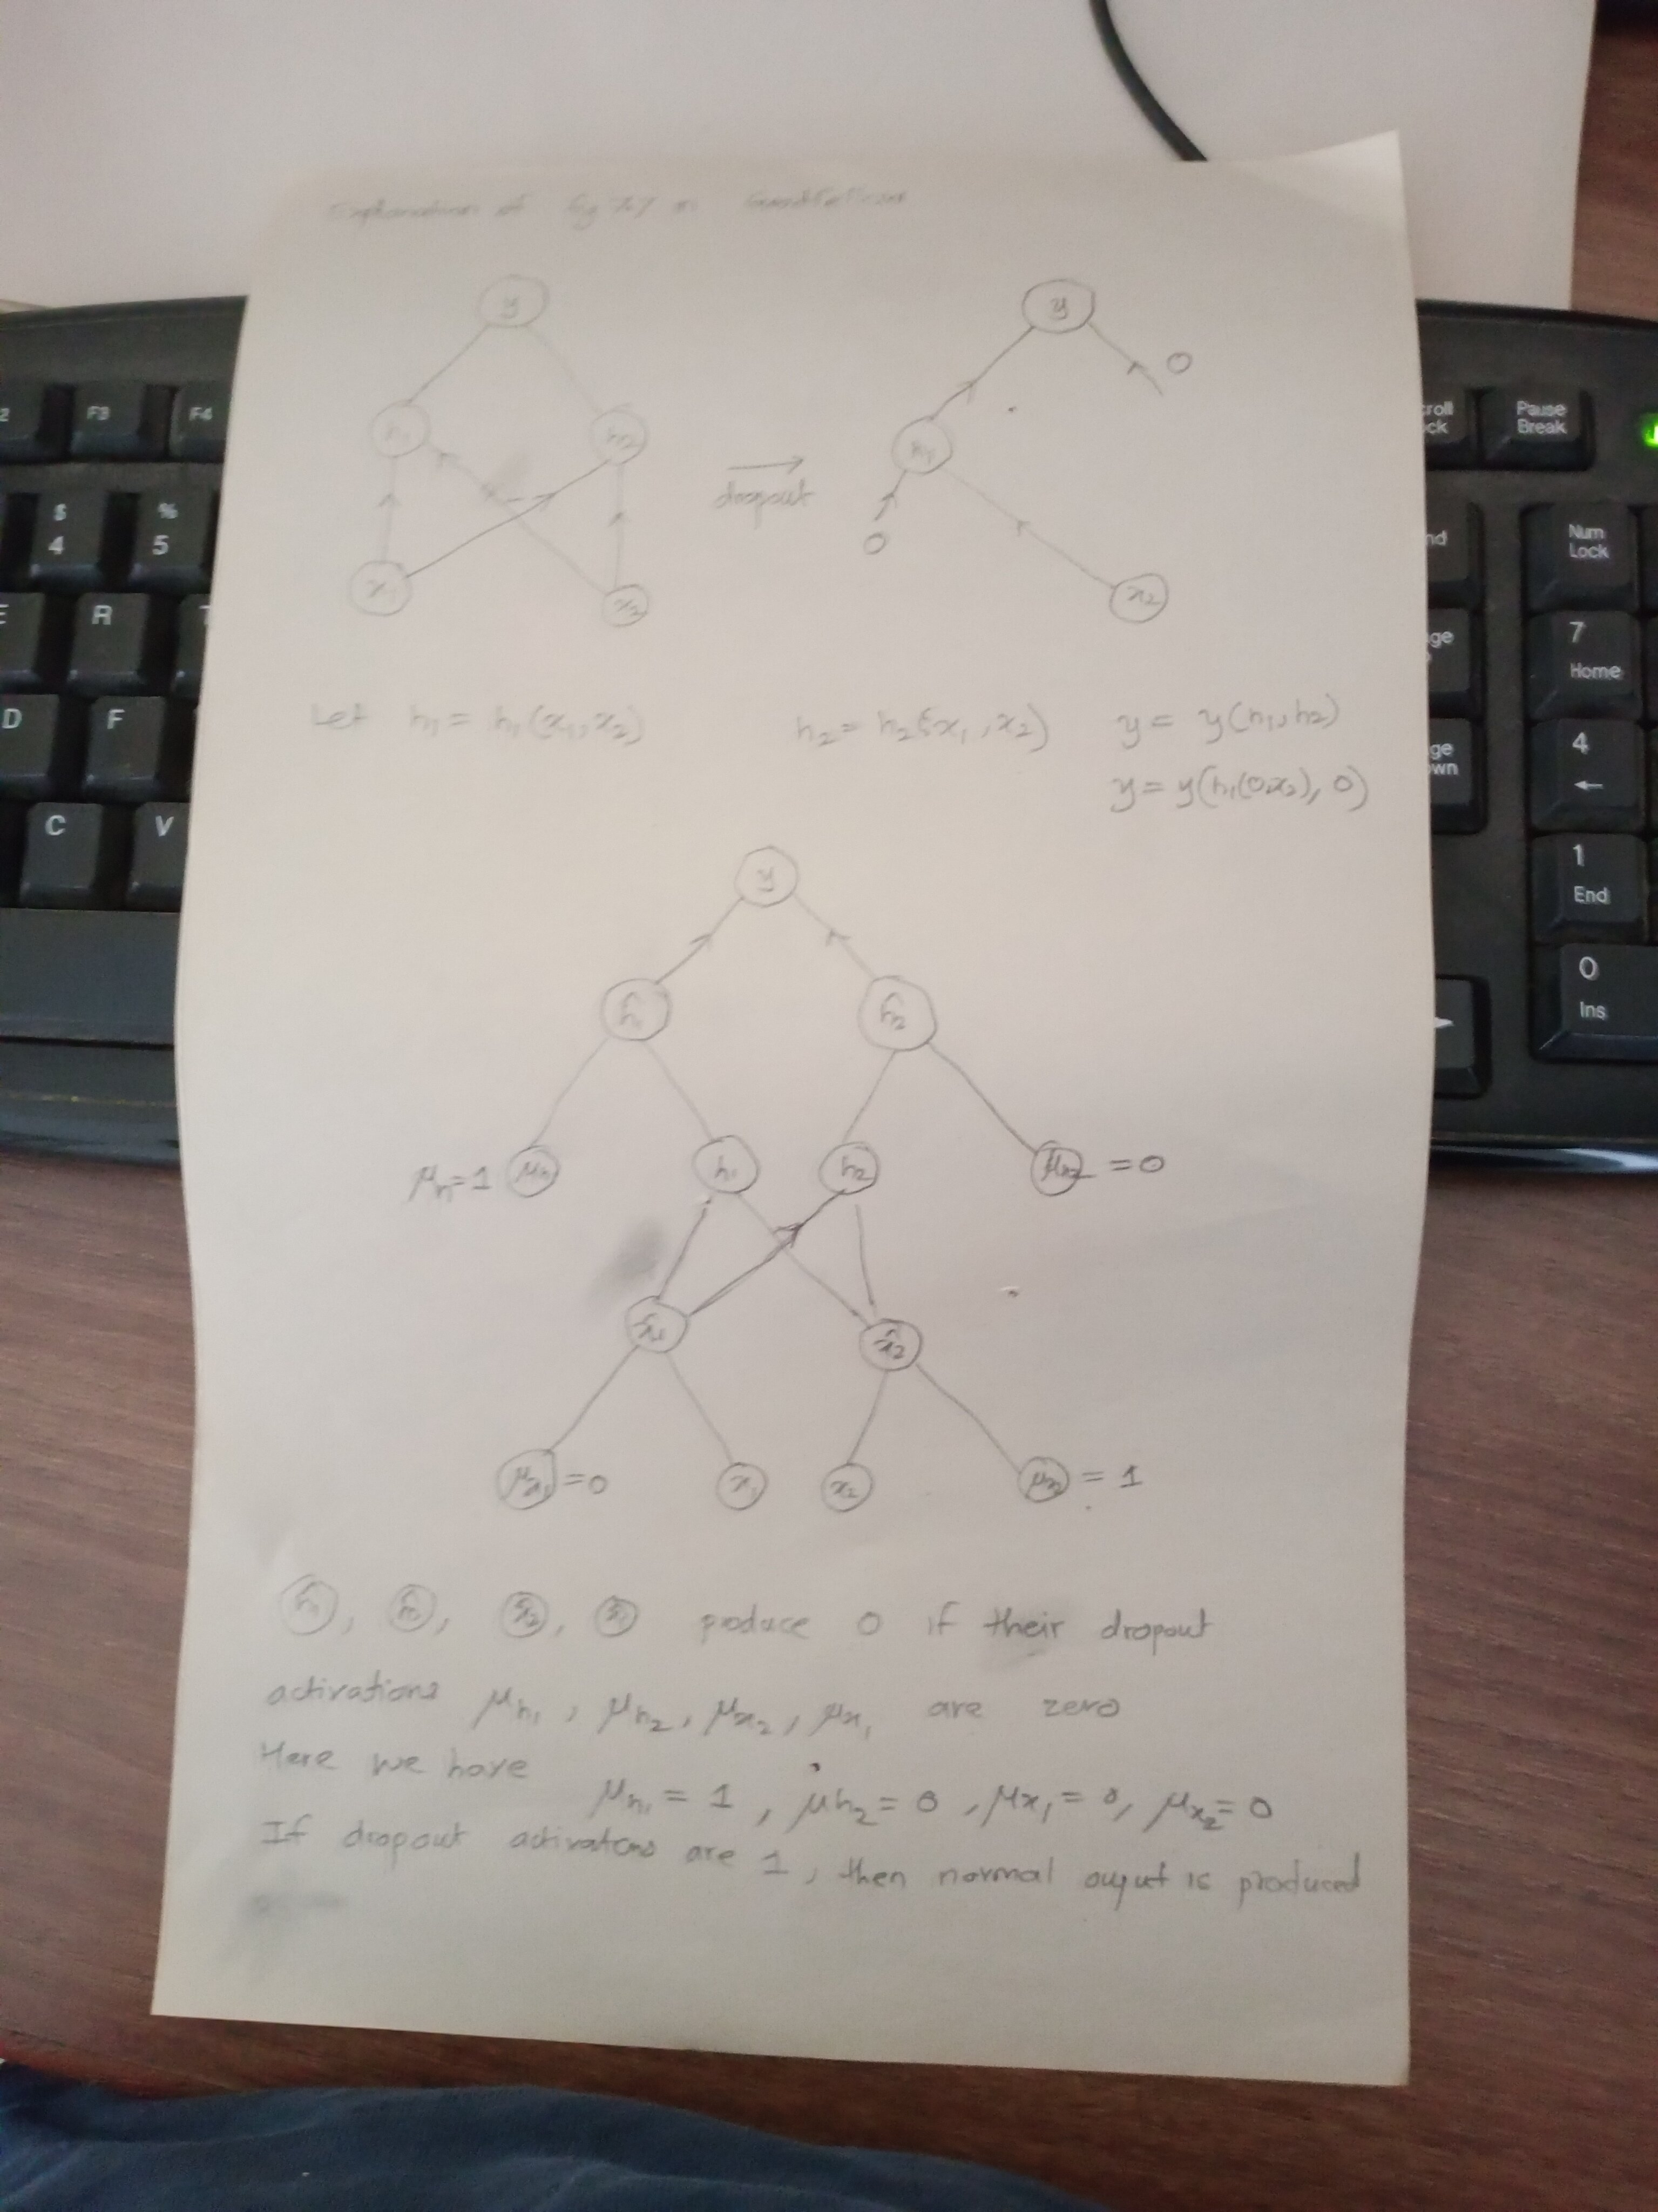
\includegraphics[width=14cm]{goodfellow_fig/dropout_fig_77.jpg}
\caption{\label{fig:goodfellow77} Explanation of figure 7.7 in Goodfellow}
\end{figure}  
%
%
%
\section{Exactness of Weight scaling inference rule}
Equation 7.65 in Goodfellow is
\beq
\exp\Big{(}\frac{1}{2^n}\sum_{\pmb{d}\in\{0,1\}^n}\pmb{W}_{y}^T(\pmb{d}\odot\pmb{v})+b_y\Big{)}
\eeq
Note: since there are no nonlinear hidden units, the output of unit $y$ which predicts class $y$ can be expressed as a vector $\pmb{W}_{y}^T$ times $\pmb{d}\odot\pmb{v}$ where the $\odot$ represents element-wise vector product. Dropout is applied only to the input. So the input becomes $\pmb{d}\odot\pmb{v}$, where $\pmb{d}\in\{0,1\}^n$. There are $2^n$ vectors corresponding to $\{0,1\}^n$. So we have,
\beq
\sum_{\pmb{d}\in\{0,1\}^n} b_y  = 2^nb_y
\eeq
Furthermore,
\beq
\sum_{\pmb{d}\in\{0,1\}^n}\pmb{W}_{y}^T(\pmb{d}\odot\pmb{v}) = \pmb{W}_{y}^T\sum_{\pmb{d}\in\{0,1\}^n}(\pmb{d}\odot\pmb{v})
= \pmb{W}_{y}^T\Big{(}\sum_{\pmb{d}\in\{0,1\}^n}\pmb{d}\Big{)}\odot\pmb{v}
= \pmb{W}_{y}^T\Big{(}2^{n-1}\Big{)}\pmb{v} = 2^{n-1}\pmb{W}_{y}^T\pmb{v}
\eeq
Where we have used
\beq
\sum_{\pmb{d}\in\{0,1\}^n}(\pmb{d}\odot\pmb{v}) = 2^{n-1}\pmb{v} \text{ which follows from }\sum_{\pmb{d}\in\{0,1\}^n}{\pmb{d}}=2^{n-1}
\eeq
So, the first equation becomes
\beq
\exp\Big(\frac{1}{2^n}(2^{n-1}\pmb{W}_{y}^T\pmb{v}+2^nb_y)\Big) = \exp\Big(\frac{1}{2}\pmb{W}_{y}^T\pmb{v}+b_y\Big) 
\eeq
So, basically, after applying dropout with probablity $0.5$ (the weights are multiplied by 1 50\% of the time, or by 0 the remaining 50\% of the time) the weights are halved. All the weight states that can be achieved by this multiplication by can be represented by $\pmb{d}\odot\pmb{v}$ for some $\pmb{d}\in\{0,1\}^n$.
%
%
%
\section{Dropout and Bagging: 7.12 }
- \textbf{Bagging (Bootstrap Aggregating)} train a separate model for each class and then ensemble the prediction\\
- \textbf{Boosting}: Construct an ensemble with higher capacity than individual models.\\
- \textbf{Dropout}: A method of making bagging practical. Instead of training multiple neural networks on different datasets and averaging, dropout trains all sub-networks of a model. Since there are a very large number of all sub-networks of a model, it is impractical to train them all. So we just sample the gradients by training a few models.\\
- \textbf{weight scaling inference rule} allows us to approximate $p_{ensemble}$ by multiplying the weights with probability of includig the link.\\
- \textbf{dropout boosting} traditional boosting increases the capacity of bagging. dropout boosting reduces the regularizing effect and thus in some sense increases capacity. (increasing regularization reduces capacity, therefore decreasing regularization increases capacity)
%
%
%
\section{\label{sect:tangentprop}Tangent prop: sect 7.14}
Let all points belonging to class $y^1$ belong to manifold $M_1$. The point of the condition 7.67 is to make sure that our prediction $f(\pmb{x})$ changes very-little as the data point moves from location $\pmb{x}_1$ on the manifold to another point $\pmb{x}_2$ closeby. If we want $f(\pmb{x})$ to change very-little along the manifold tangent vectors, then we want to make the component of the gradient along the tangnet vectors zero. That is the gradient should be orthogonal to the tangent vectors. Equation 7.67 penalizes the derivative along tangent vectors.
%
%
%
\section{Stochastic gradient descent: ph 280}
SGD reduces computational cost\\
SGD might get out of local minima because of the noise introduced \url{https://leon.bottou.org/publications/pdf/nimes-1991.pdf}\\
SGD follows gradient of the true generalization error as long as no examples are repeated.\\
%
%
%
\section{Optimization: 8.2 Why maximize ecpectations}
Goodfellow et al seem to prefer minimizing the expectation of some loss function over the data generating distribution as shown in equation 8.2. This is because taking the expectation automatically assigns higher weight to high-probability examples, and lower weight to lower probability examples.
%
%
%
\section{Saddle points and local minima: sect 8.2.3}
There are many more saddle points than local minima. `''To understand the intuition behind this behavior, observe
that the Hessian matrix at a local minimum has only positive eigenvalues. The
Hessian matrix at a saddle point has a mixture of positive and negative eigenvalues.
Imagine that the sign of each eigenvalue is generated by flipping a coin. In a single
dimension, it is easy to obtain a local minimum by tossing a coin and getting heads
once. In n-dimensional space, it is exponentially unlikely that all n coin tosses will`''\\

Newton's method is explicitly designed to seek points of zero gradient. Saddle points satisfy the condition of zero gradient. Newton's method may seek out saddle points. Saddle-free Newton methods exist.

%
%
%
\section{Equation 8.14}
\ber
\epsilon_k = (1-\alpha)\epsilon_0 + \alpha\epsilon_{\tau}
\eer
Here, $\epsilon_{\tau}$ is to be interpreted as a fixed constant.

\section{Sect 8.3.1: Advice on learning rate}
`''Typically, the optimal initial learning rate, in terms of total training time and the
final cost value, is higher than the learning rate that yields the best performance
after the first 100 iterations or so. Therefore, it is usually best to monitor the first
several iterations and use a learning rate that is higher than the best-performing
learning rate at this time, but not so high that it causes severe instability.`''
%
%
%
\section{Optimization with momentum: section 8.3.2}
It is less important to adapt $\alpha$ (momentum parameter) time than to shrink $\epsilon$ (learning rate)  over time.


%
%
%

\section{Sect 8.4 Parameter initialization strategies}
`''A good rule of thumb for choosing the initial scales is to
look at the range or standard deviation of activations or gradients on a single
minibatch of data. If the weights are too small, the range of activations across the
minibatch will shrink as the activations propagate forward through the network.
By repeatedly identifying the first layer with unacceptably small activations and
increasing its weights, it is possible to eventually obtain a network with reasonable
initial activations throughout.`''

%
%
%

\section{Section 8.4 weight initialization}
`''We can think of initializing the parameters $\pmb{\theta}$ to $\pmb{\theta}_0$ as being similar to imposing a Gaussian prior $p(\pmb{\theta})$ with mean $\pmb{\theta}_0$
%
%
%
\section{Section 8.4 Marginal mean}
\url{https://stats.stackexchange.com/questions/4245/what-is-the-meaning-of-marginal-mean} Marginal mean is the mean of a marginal distribution. A marginal distribution is defined in expectation\_probability.tex
%
%
%
\section{Section 8.5.2 RMSProp: recurrence relation}
From \url{https://en.wikipedia.org/wiki/Stochastic_gradient_descent#RMSProp}.\\
\ber
v_{t} = \gamma{}v_{t-1} + (1-\gamma)(\nabla{Q_t}^2)
\eer
$v_{0}$ is probably initialized to the first gradient or maybe even to zero
\ber
v_{t} &=& \gamma{}(\gamma{}v_{t-2}+(1-\gamma)(\nabla{Q_{t-1}})^2) + (1-\gamma)(\nabla{Q_t})^2\\
&=& \gamma^2v_{t-2} + \gamma(1-\gamma)(\nabla{Q_{t-1}})^2 + (1-\gamma)(\nabla{Q_t})^2\\
&\approx& \sum_{k=0}^{t}\gamma^{k}(1-\gamma)(\nabla{Q_{t-k}})^2
\eer
This shows the exponential weighting to the older gradients.

%
%
%
\section{Batch normalization section 8.7}
1) Small updates to weights can cause large changes in the output due to adding up of second order effects\\
2) Higher order optimizations can take into account the second and higher order effects but these optimization algos are very expensive\\
3)`''Batch normalization provides an elegant way of reparametrizing almost any deep
network. The reparametrization significantly reduces the problem of coordinating
updates across many layers.`''\\
4) Can be thought of as eliminating linear interactions
%
%
%
\section{CNNs equivariance}
CNNs are equivariant to translations but not rotation and scaling.
%
%
%
\section{Recurrent Neural Networks: equation 10.14}
Note: this equation is like the maximum likelihood as before in Section (\ref{sect:mle}). What exactly Goodfellow means by `''where $p_{model}$ is given by reading the entry for $y^{(t)}$ from the
model’s output vector $\hat{\pmb{y}}ˆ{(t)}$`'' is unknown, but it is somemethod of of calculating/approximating $p_{model}$.
%
%
%
\section{Recurrent Neural Networks: equation 10.15/10.16}
\ber
p(A\cap{B}) = p(A|B)p(B) = p(B|A)p(A)
\eer
This theorem works even when we are in a probability space in which $x_1,x_2$ is true. That is, when we are given $x_1,x_2$. So,
\ber
p(y^1,y^2|x^2,x^1) = p(y^2|y^1,x^1,x^2)p(y^1|x^1,x^2)
\eer
If we want to be pedantic, note
\beq
p(y^2|y^1|x^1,x^2) = p(y^2|y^1,x^1,x^2)
\eeq
%
%
%
\section{Encoder decoder Sequence-to-Sequence Architectures}
Fig 10.12 - Not clear where the loss is calculated. Has to be after y is calculated. For an example see \url{https://keras.io/examples/nlp/lstm_seq2seq/}.
%
%
%
\section{Dynamics of forward and backpropagation: p.g. 406}
`''Note that it is possible for back-propagation to retain unbounded dynamics even when forward propagation has bounded dynamics,`''\\
Consider the following NN
\ber
w_1 = \tanh{a_1x} \qquad y = \tanh{a_2w_1}
\eer
The output $y$ is bounded because $\tanh$ is bounded. Backpropagation for the derivatives gives
\ber
\pdd{y}{w_1} = (1-\tanh^2{(a_2w_1)})a_2\\
\pdd{w_1}{x} = (1-\tanh^2{(a_1x)})a_1\\
\pdd{y}{x} = (1-\tanh^2{(a_2w_1)})(1-\tanh^2{(a_1x)})a_1a_2
\eer
So the $a_1$ and $a_2$ come as a product in derivative. In deep neural networks with multple layers, this product may cause derivatives to become unbounded or vanish depending on whether all $a_i>0$ or all $a_i<0$. When multiple units per layer are present, the $a_i$ become the eigenvalues of the jacobian of the transformation. 
%
%
%
\section{Bayes' error section 11.1}
\url{https://en.wikipedia.org/wiki/Bayes_error_rate} `''In statistical classification, Bayes error rate is the lowest possible error rate for any classifier of a random outcome (into, for example, one of two categories) and is analogous to the irreducible erro`''\\
Goodfellow p.g. 131 `''The ideal model is an oracle that simply knows the true probability distribution
that generates the data. Even such a model will still incur some error on many
problems, because there may still be some noise in the distribution. In the case
of supervised learning, the mapping from $\pmb{x}$ to $\pmb{y}$ may be inherently stochastic,
or $\pmb{y}$ may be a deterministic function that involves other variables besides those
included in $\pmb{x}$. The error incurred by an oracle making predictions from the true
distribution $p(\pmb{x}, \pmb{y})$ is called the Bayes error`''
%
%
%
\section{Precision and recall section 11.1}
\url{https://en.wikipedia.org/wiki/Precision_and_recall#Precision}
\ber
\text{Precision} = \frac{tp}{tp+fp} \qquad \text{Recall} = \frac{tp}{tp+fn}
\eer
in case denominators go to zero, we can control the behavior using \textit{zero\_division} in sklearn. \url{https://scikit-learn.org/stable/modules/generated/sklearn.metrics.precision_score.html}
%
%
\section{F-score}
\ber
F_1 = 2\frac{\text{precision}\text{recall}}{\text{precision}+\text{recall}}
\eer
In general higher, F-score is better. Depends on how you want to trade-off precision and recall.
%
%
%
\section{Collecting more data sect 11.3}
- If training set data is not being used (underfit), do not collect more data\\
- If test set perf is much worse than training set perf collect more data. An explanation of this is that we need more data to learn features that will generalize.

\section{Test set error sect 11.4 pg 430}
`''The test error is the sum of the training error and the gap between training and test error.`'' We want to keep the training error constant and decrease the gap between the training and test error.
%
%
%
\section{Grid search 11.4.3}
Because we provide pdfs to random search, we end up concentrating our efforts in the region where we believe good hyperparameters are present. Grid search ends up exploring unimportant parameter spaces as well. Of course, we must have good pdfs for random search.
%
%
%
\section{Section 12.2.1.1 Gradient contrast normalization eqn 12.3}
I can't see how equation 12.3 projects points to the sphere. The denominator is constant, the numerator is purely a shift in coordinates. To do what they claim it does, it needs to be non-linear methinks
%
%
%
\section{Autoencoders pg 516 sect 14.6}
``only the variations tangent to the manifold around x need to correspond to changes in h = f(x).'' This appears to be a contradiction to section (\ref{sect:tangentprop}). The difference here seems to be that the autoencoder has to learn that the tangent directions are important parts of representation of $x$, because the label does not change along them. $f$ for autoencoders is the encoding function and not the output label. In section (\ref{sect:tangentprop}) $f$ is the output label (which we do not want to change along the tangent directions).

%
%
%
\end{document}

